\chapter{TINJAUAN PUSTAKA}
\section{\textit{Internet of Things}}
\tab \textit{Internet of Things} (IoT) adalah sebuah konsep komputasi yang menggambarkan sebuah gagasan tentang objek fisik sehari-hari yang terhubung ke internet dan mampu mengidentifikasi diri mereka ke perangkat lain. Istilah ini erat diidentifikasi oleh RFID sebagai metode komunikasi antar objek tanpa melibatkan interaksi manusia ke manusia atau manusia ke komputer, termasuk teknologi sensor, \textit{wireless}, atau \textit{QR codes}. IoT telah berkembang dari konvergensi teknologi nirkabel, \textit{micro-electromechanical systems} (MEMS), dan internet.\\
\tab IoT adalah signifikan, karena sebuah objek dapat merepresentasikan dirinya secara digital menjadi sesuatu yang lebih besar dari objek itu sendiri. Objek tidak hanya bisa berhubungan dengan pengguna, namun objek dapat terhubung dengan objek lain disekitarnya dan dengan basis data. Ketika banyak objek bekerja bersama-sama sebagai satu kesatuan, maka mereka memiliki kecerdasan yang disebut \textit{"ambient intelligence"}.\\
\tab \textit{Internet of Things} adalah konsep yang sulit didefinisikan secara tepat sebab penelitian pada IoT masih dalam tahap perkembangan. Bahkan ada banyak kelompok yang berbeda yang telah mendefinisikan istilah tersebut, meski penggunaan awal istilah ini dikaitkan dengan Kevin Ashton, seorang pakar inovasi digital. Ada sebuah pernyataan Ashton (1999) yang dikutip dari sebuah artikel di \textit{RFID Journal}:\\
\tab \textit{"Jika kita memiliki komputer yang tahu segalanya yang harus diketahui dari berbagai benda \textit{(things)} – menggunakan data yang mereka kumpulkan sendiri tanpa bantuan dari kita – kita bisa melacak dan menghitung semuanya, serta sangat mengurangi pemborosan, kerugian, dan biaya. Kita bisa tahu kapan suatu benda perlu diganti dan diperbaiki, atau kapan benda-benda itu masih dalam kondisi baik."}\\
\tab IoT menggambarkan sebuah dunia dimana hampir semua hal dapat terhubung dan berkomunikasi. Dengan kata lain, dengan \textit{Internet of Things}, dunia akan menjadi satu kesatuan sistem informasi yang sangat besar. \textit{Internet of Things} memiliki potensi untuk mengubah dunia seperti pernah dilakukan oleh internet, bahkan mungkin lebih baik (Ashton, 2009).

\section{Mikrokontroler dan Komponen Elektronika}
\tab Mikrokontroler adalah komputer kecil pada satu sirkuit terintegrasi yang berisi prosesor, memori, dan beberapa pin \textit{input/output} yang bisa dikontrol (sering disebut GPIO (\textit{General Purpose Input Output Pins})).

\subsection{Arduino UNO}
\tab Arduino UNO adalah sebuah papan mikrokontroler \textit{open-source} berbasis \textit{microchip} ATmega328 dan dikembangkan oleh Arduino.cc.\cite{arduino-uno} Papan ini dilengkapi dengan pin \textit{input/output} (I/O) digital dan analog yang dapat dihubungkan ke berbagai sirkuit lainnya. Arduino UNO mempunyai 14 pin digital, 6 pin analog, sebuah osilator Kristal 16 MHz, sebuah koneksi USB, sebuah \textit{power jack}, sebuah ICSP \textit{header}, dan sebuah tombol reset. Gambar \ref{figure:arduino-uno-pinout} menunjukkan komponen papan Arduino UNO.\\
\tab Papan Arduino juga dapat diprogram menggunakan \textit{software} Arduino IDE (Lingkungan Pengembangan Terpadu) melalui kabel USB tipe B dan dapat disuplai melalui koneksi USB atau dengan baterai eksternal 9 volt, walaupun Arduino sebenarnya dapat menerima voltase 7 hingga 20 volt.

\begin{figure}[H]
	\centerline {
		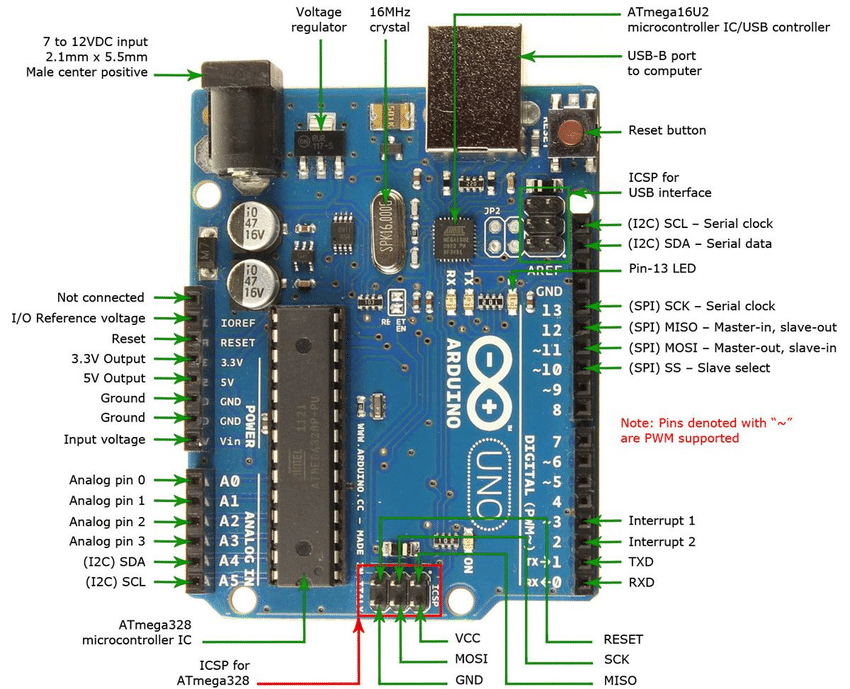
\includegraphics[width=\linewidth]{bab3/img/arduino-uno-pinout.png}
	}
	\caption{Komponen Papan Arduino UNO}
	\label{figure:arduino-uno-pinout}
\end{figure}

\subsection{ESP8266-01}
\tab ESP8266 adalah sebuah \textit{System On Chip} (SOC) yang memiliki kemampuan untuk terhubung dengan jaringan TCP/IP via Wi-Fi. Selain itu, ESP8266 juga memiliki kemampuan layaknya mikrokontroler, yakni sebagai sebuah “otak” dan  pengendali dalam dunia elektronika \textit{embedded}, sehingga ESP8266 dapat diprogram langsung tanpa memerlukan mikrokontroler tambahan. \\
\tab Modul Wi-Fi ini dibuat oleh \textit{Espressif System}, pabrikan asal Cina. Produk seri ESP8266 memiliki banyak sekali varian, salah satunya adalah ESP8266 seri ESP-01. Gambar \ref{figure:ESP8266-01} menunjukkan \textit{pinouts} dari ESP8266-01.

\begin{figure}[H]
	\centerline {
		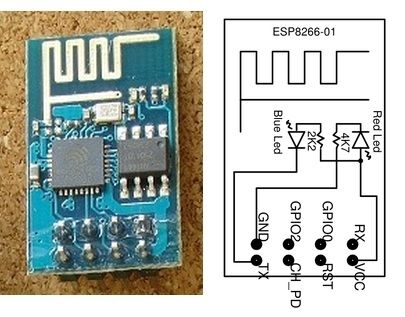
\includegraphics[width=\linewidth]{bab3/img/ESP8266-01.jpg}
	}
	\caption{\textit{Pinouts} ESP8266-01}
	\label{figure:ESP8266-01}
\end{figure}

\subsection{DHT11}
\tab DHT11 adalah salah satu sensor yang dapat mengukur dua parameter lingkungan sekaligus, yakni suhu dan kelembaban udara. Dalam sensor ini, terdapat sebuah \textit{thermistor} tipe NTC \textit{(Negative Temperature Coefficient)} untuk mengukur suhu, sebuah sensor kelembaban tipe resistif, dan sebuah mikrokontroler 8-bit yang mengolah kedua sensor tersebut dan mengirim hasilnya ke pin \textit{output} dengan format \textit{single-wire bi-directional} (kabel tunggal dua arah). Gambar \ref{figure:pinout-DHT11} menunjukkan \textit{pinouts} dari DHT11.

\begin{figure}[H]
	\centerline {
		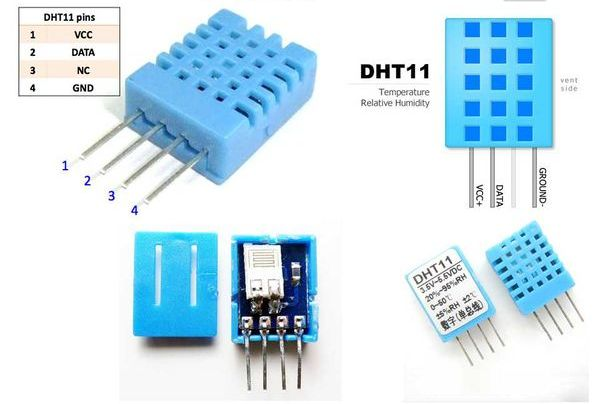
\includegraphics[width=\linewidth]{bab3/img/pinout-DHT11.jpg}
	}
	\caption{\textit{Pinouts} DHT11}
	\label{figure:pinout-DHT11}
\end{figure}

\textbf{Keterangan:}
\begin{itemize}
	\item Pin 1 : Vcc 3.5 – 5.5V DC
	\item Pin 2 : DATA/serial data \textit{(single bus)}
	\item Pin 3 : NC, \textit{not used}
	\item Pin 4 : GND/\textit{ground}
\end{itemize}

\subsection{\textit{Infrared Sensor Module} dan \textit{Infrared Receiver Module}}
\tab \textit{Infrared sensor module} pendeteksi objek/hambatan adalah komponen elektronik yang memancarkan sinar inframerah untuk mendeteksi atau merasakan beberapa aspek di sekitarnya. Sensor inframerah dapat mengukur suhu suatu objek ataupun mendeteksi gerakan objek. Komponen ini mengeluarkan \textit{output} berupa sinyal digital sehingga mudah digunakan untuk berinteraksi dengan mikrokontroler terkenal seperti Arduino/Genuino UNO, ESP8266, Mega, Leornado, Zero, 101, bahkan Raspberry Pi atau Raspberry Pi Zero.\\

\begin{figure}[H]
	\centerline {
		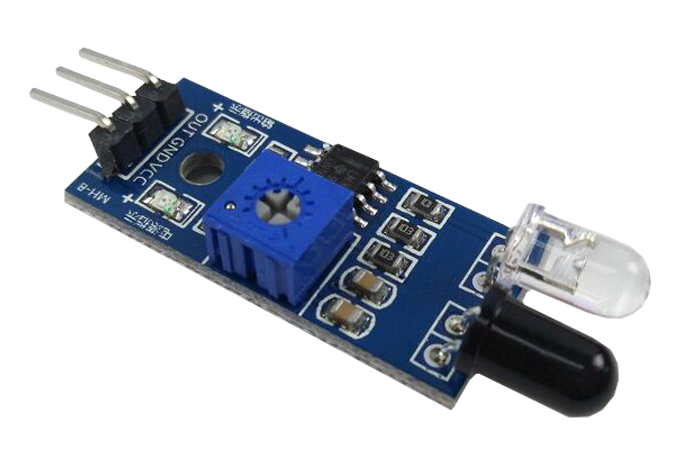
\includegraphics[height=3cm]{bab3/img/ir-sensor.png}
		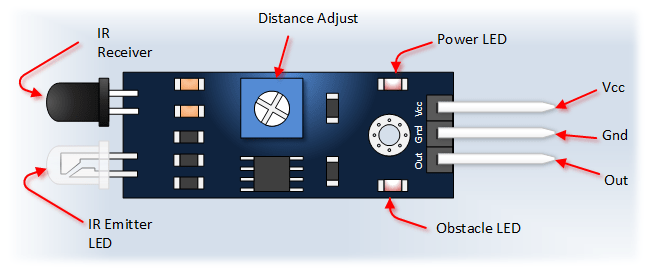
\includegraphics[height=3cm]{bab3/img/ir-sensor-pin.png}
	}
	\caption{\textit{Infrared Sensor Module}}
	\label{figure:ir-sensor}
\end{figure}

Seperti yang ditunjukkan pada gambar \ref{figure:ir-sensor}, modul ini memiliki sepasang pemancar dan penerima sinar inframerah di bagian depan modul, pemancar berupa sebuah LED \textit{(Light-Emitting Diode)} inframerah dan penerima berupa sebuah \textit{photodiode} yang sensitif terhadap cahaya inframerah dengan panjang gelombang yang sama dengan yang dipancarkan oleh LED. Setiap kali ada objek yang berada di depan LED pemancar, maka objek tersebut akan memantulkan sinar inframerah dan penerima akan menangkap sinar tersebut. \\
\tab Selain jenis sensor inframerah di atas, ada pula jenis sensor yang hanya mengukur sinar inframerah tanpa memancarkannya, disebut dengan \textit{infrared receiver module} yang hanya terdiri dari \textit{photodiode} sebagai penerima sinyal inframerah. Ada banyak sekali jenis \textit{infrared receiver}, salah satunya adalah jenis 1838b berikut deskripsi pin nya pada gambar \ref{figure:ir-receiver4}.

\subsection{\textit{Breadboard}}
\tab Breadboard atau yang juga biasa disebut \textit{Project Board} adalah dasar konstruksi sebuah sirkuit elektronik untuk membuat prototipe dari suatu rangkaian elektronik. Breadboard banyak digunakan untuk membuat prototipe suatu rangkaian komponen elektronik karena dalam penggunaannya tidak memerlukan proses menyolder \textit{(solderless)} sehingga mudah digunakan. Breadboard dapat digunakan kembali dan sangat cocok digunakan untuk berkreasi dalam desain sirkuit elektronika. Secara umum, breadboard memiliki jalur seperti pada gambar \ref{figure:breadboard_scheme}.

\begin{figure}[H]
	\centerline {
		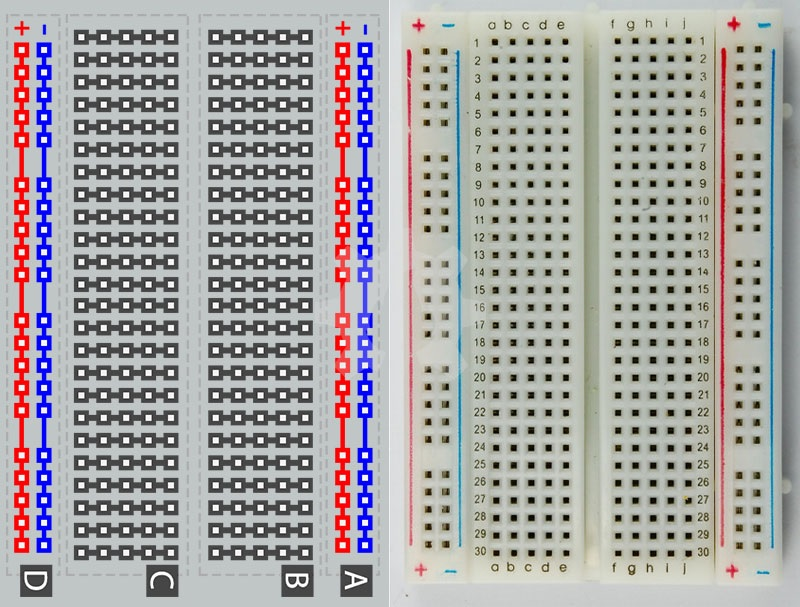
\includegraphics[width=\linewidth]{bab3/img/breadboard.jpg}
	}
	\caption{Breadboard}
	\label{figure:breadboard_scheme}
\end{figure}

\subsection{Resistor}
\tab Resistor merupakan komponen elektronik yang memiliki dua pin dan didesain untuk mengatur tegangan dan arus listrik. Resistor mempunyai nilai resistansi (tahanan) tertentu yang dapat memproduksi tegangan listrik di antara kedua pin dimana menurut persamaan hukum \textit{Ohm} seperti pada gambar \ref{figure:hukum-ohm}, nilai tegangan terhadap resistansi berbanding lurus dengan arus listrik yang mengalir.

\begin{figure}[H]
	\centerline {
		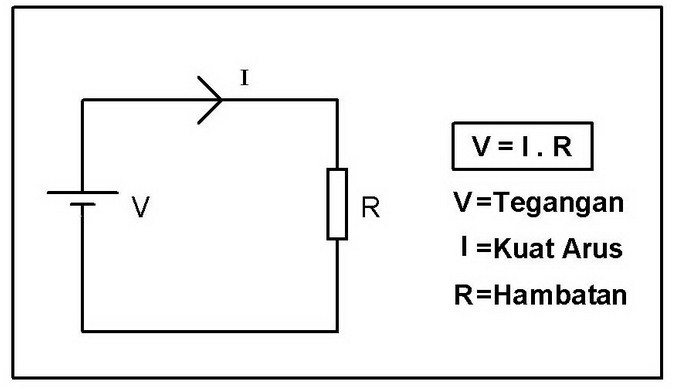
\includegraphics[height=4cm]{bab3/img/hukum-ohm.jpg}
	}
	\caption{Hukum \textit{Ohm}}
	\label{figure:hukum-ohm}
\end{figure}

Resistor digunakan sebagai bagian dari rangkaian elektronik dan sirkuit elektronik, serta merupakan salah satu komponen yang paling sering digunakan. 

\subsection{\textit{Jumper Wires}}
\tab \textit{Jumper wires} atau kabel \textit{jumper} adalah kabel yang memiliki konektor atau pin pada masing-masing ujungnya. \textit{Jumper wires} biasanya digunakan untuk menghubungkan antar komponen \textit{breadboard} atau dengan prototipe sirkuit elektronik lain. Sama seperti \textit{breadboard}, \textit{jumper wires} dapat digunakan tanpa menyolder \textit{(solderless)}. Ada 3 macam kabel \textit{jumper} berdasarkan jenis ujung kabelnya, yakni \textit{male to male}, \textit{male to female}, dan \textit{female to female} yang ditunjukkan pada gambar \ref{figure:jumperwires}

\begin{figure}[H]
	\centerline {
		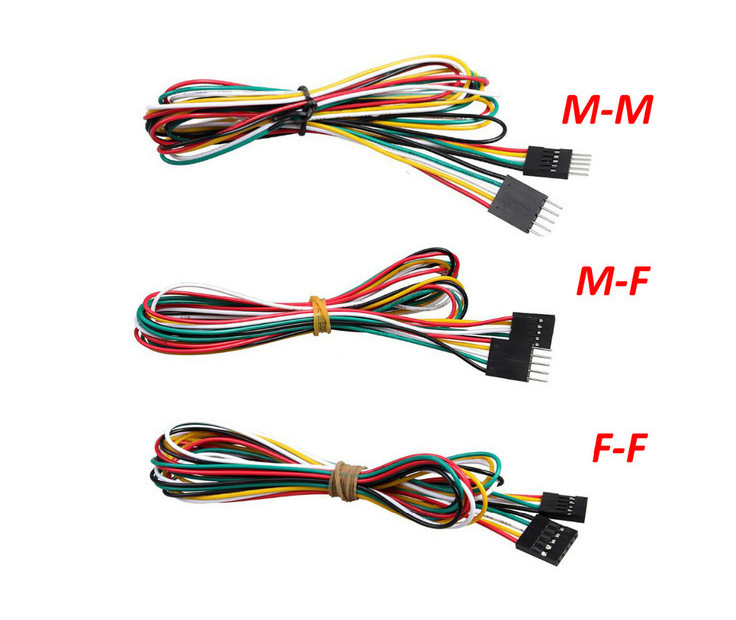
\includegraphics[width=\linewidth]{bab3/img/jumperwires.png}
	}
	\caption{Jenis \textit{Jumper Wires}}
	\label{figure:jumperwires}
\end{figure}
 
\subsection{Lampu LED}
\tab Lampu LED adalah produk \textit{Light-Emitting Diode} (LED) yang disusun menjadi sebuah bola lampu. Lampu LED memiliki usia pakai dan efisiensi listrik lebih baik daripada lampu pijar, serta jauh lebih efisien daripada lampu neon. Lampu LED juga merupakan salah satu komponen yang sering digunakan dalam rangkaian mikrokontroler karena bohlam LED dapat dijadikan sebagai parameter keberhasilan sebuah rangkaian, misalnya pada rangkaian yang menggunakan komponen sensor untuk memberikan \textit{trigger} supaya lampu LED menyala.


\begin{figure}[H]
	\centerline {
		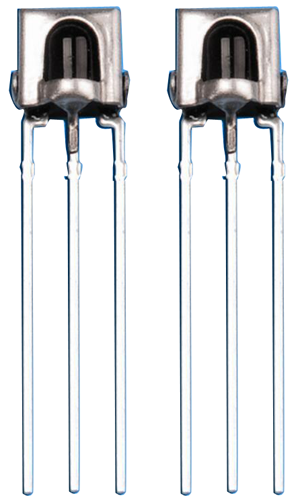
\includegraphics[height=6cm]{bab3/img/ir-receiver2.png}
		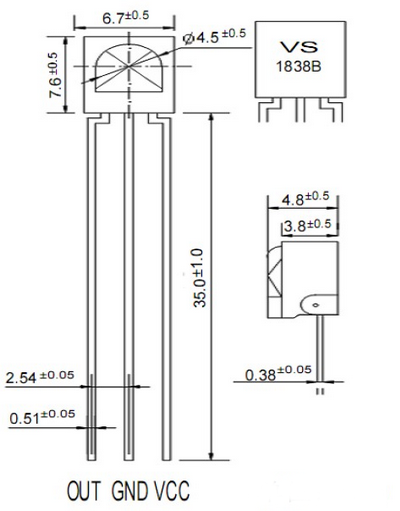
\includegraphics[height=6cm]{bab3/img/ir-receiver4.png}
	}
	\caption{\textit{Infrared Receiver Module}}
	\label{figure:ir-receiver4}
\end{figure}

\section{Pemrograman Mikrokontroler}
\tab Ada banyak sekali bahasa pemrograman yang dapat digunakan untuk memprogram suatu mikrokontroler, seperti BASIC, C/C++, atau Assembly (ASM). Arduino sendiri memiliki sebuah perangkat pemrograman bernama Arduino IDE yang dapat digunakan untuk membuat program menggunakan bahasa C yang memang sudah dirancang khusus untuk Arduino. 

\subsection{Bahasa Pemrograman C}
\tab Bahasa pemrograman C adalah bahasa pemrograman tingkat menengah yang bisa digunakan untuk membuat berbagai jenis aplikasi, mulai dari sistem operasi hingga \textit{compiler} untuk bahasa pemrograman lain. Bahasa pemrograman yang dibuat oleh Dennis M. Ritchie pada tahun 1972 ini paling cocok digunakan untuk membangun aplikasi yang berhubungan langsung dengan sistem operasi dan \textit{hardware}. Bahasa pemrograman C inilah yang digunakan untuk memprogram papan Arduino dan menghubungkannya dengan Telegram Bot API.\\

\subsection{Arduino IDE}
\tab Arduino IDE atau Arduino \textit{Software} (IDE) adalah sebuah \textit{software open-source} yang memungkinkan pengembang untuk menulis kode program dan mengunggahnya ke papan Arduino. Unit kode yang diunggah dan dijalankan di papan Arduino biasa disebut dengan Sketsa atau \textit{Sketch}. Arduino IDE dapat berjalan di sistem operasi Windows, Linux, maupun Mac OS X dan dapat digunakan bersama papan Arduino jenis apapun. 

\section{Telegram}
\tab Telegram adalah sebuah aplikasi \textit{messaging} yang fokus pada kecepatan dan keamanan, sederhana, ringan, dan juga gratis. Telegram yang diluncurkan pada Agustus tahun 2013, menjadi salah satu aplikasi \textit{instant messaging} yang banyak digunakan oleh masyarakat di seluruh dunia. Kelebihan Telegram salah satunya adalah adanya landasan untuk menggunakan \textit{Application Programming Interface} (API) untuk
masyarakat luas.

\subsection{Telegram Bot API}
\tab Telegram menyediakan dua jenis API yang dapat dikembangkan, yakni  Telegram API dan Bot API.\cite{telegram} Telegram API adalah API yang memungkinkan siapa saja membuat klien Telegram mereka sendiri sesuai dengan keinginan. Telegram adalah aplikasi yang \textit{open source} karena \textit{source code}-nya disebarluaskan secara luas dan gratis untuk dipelajari dan dibuka 100\% untuk para pengembang yang ingin membuat aplikasi Telegram menggunakan \textit{platform} mereka. \\
\tab Bot API adalah sebuah API yang memungkinkan siapa saja dengan mudah membuat sebuah program yang menggunakan aplikasi Telegram sebagai antarmuka.\cite{telegram-bot} Bot API memungkinkan siapa saja untuk membuat bot (kependekan dari robot) yang dapat membalas dan melayani semua pengguna yang mengirimkan suatu pesan perintah kepada bot tersebut. \\
\tab Bot adalah aplikasi pihak ketiga yang dijalankan di dalam Telegram dan dioperasikan oleh perangkat lunak, bukan manusia. Bot dapat melakukan apa saja, seperti mengajari, mencari, \textit{broadcast}, mengingatkan, menghubungkan, dan mengintegrasikan dengan layanan lainnya atau bahkan dapat memberikan perintah ke \textit{Internet of Things}.\\
\tab Pengguna dapat berinteraksi dengan bot dengan mengirimkan pesan, perintah, dan permintaan. Sedangkan pengembang dapat mengontrol bot yang sedang dikembangkannya melalui \textit{HTTPS Requests} ke bot API Telegram.

\section{WSO2 IoT \textit{Server}}
\tab WSO2 adalah sebuah teknologi \textit{open-source} untuk bisnis digital yang menyediakan layanan integrasi yang tangkas (\textit{agile}). Ada 3 macam layanan yang ditawarkan, yakni WSO2 \textit{Integration Agile Platform}, \textit{Architecture for Agility}, dan \textit{Methodology for Agility}. Diantara banyak produk yang ditawarkan oleh WSO2, ada salah satu \textit{platform} yang berkaitan dengan \textit{Internet of Things} bernama WSO2 \textit{IoT Server}. WSO2 \textit{IoT Server} (IoTS) menyediakan kapabilitas yang diperlukan untuk mengimplementasikan \textit{platform} IoT di sisi server yang \textit{scalable}.\\
\tab Saat ini, Telkom sedang mengembangkan WSO2 \textit{IoT Server} dan produk-produk WSO2 yang lain yang harus diuji coba. Oleh karena itu, kami mengembangkan sistem berbasis \textit{Internet of Things} yang bernama "EasyMeeting".

\cleardoublepage